\chapter{Introdução}
\label{c.introducao}

“Com o advento da realidade virtual e o avanço dos recursos computacionais, as representações interativas e imersivas do imaginário, bem como a reprodução do real, tornaram-se mais fáceis de serem obtidas. ” \cite[p. ~9]{torilivro}

A realidade virtual (RV) vem ganhando espaço em diversos setores como jogos, indústria e educação. Na área de jogos, empresas como Playstation® e Oculus® oferecem um acervo de jogos para as suas respectivas plataformas. Ao procurar por jogos em RV na Google Play, encontram-se algumas opções fornecidas por diversas empresas.

A realidade virtual pode ser utilizada na indústria para avaliar o design de um produto antes do mesmo ser produzido. A The Ford Motor Company é uma das empresas que utilizam a realidade virtual. Com esta tecnologia, é possível visualizar virtualmente tanto o exterior como o interior de um carro a ser produzido e avaliar aspectos de engenharia e design. “A realidade virtual pode ser mais efetiva do que desenvolver o design no mundo real. Só neste ano, designers e engenheiros verificaram mais de 135000 detalhes em 193 protótipos virtuais de veículos” \cite[tradução nossa]{ford}. 

Já na área da educação, a realidade virtual pode ser aplicada através de jogos educativos e aulas imersivas. Imagine uma aula de história passada no local e no tempo de um acontecimento histórico, ou uma aula de astronomia no espaço. Pesquisas como \cite{youngblut} e \cite{carvalho} mostram como a realidade virtual pode ser incorporada na escola.

Para se obter uma experiência em realidade virtual, são necessários capacetes de visualização ou óculos de RV, um display por onde a aplicação irá rodar, um dispositivo de interação e a aplicação em RV. 

Atualmente existem vários modelos de óculos de RV com suporte à realidade virtual, tais como: Oculus Rift da Oculus® com preço estimado de R\$ 4.620,90 e Samsung Gear VR da Samsung® (R\$ 799,00). No entanto, o Google Cardboard da Google® é o que possui preço mais acessível em torno de R\$ 21,97 possuindo atualmente duas versões, cada uma com um meio de interação próprio. Em novembro 2016, a Google lança um novo visualizador denominado Daydream (Figura X). Este visualizador acompanha um controle com comunicação Bluetooth e o capacete de visualização feito com tecido para garantir maior conforto, além de um suporte para fixação do visualizador à cabeça do usuário. Os smartphones compatíveis com o Daydream são os que possuem Android 7.0 ou superior.

\begin{figure}[ht]
	\caption{\small Daydream}
	\centering
	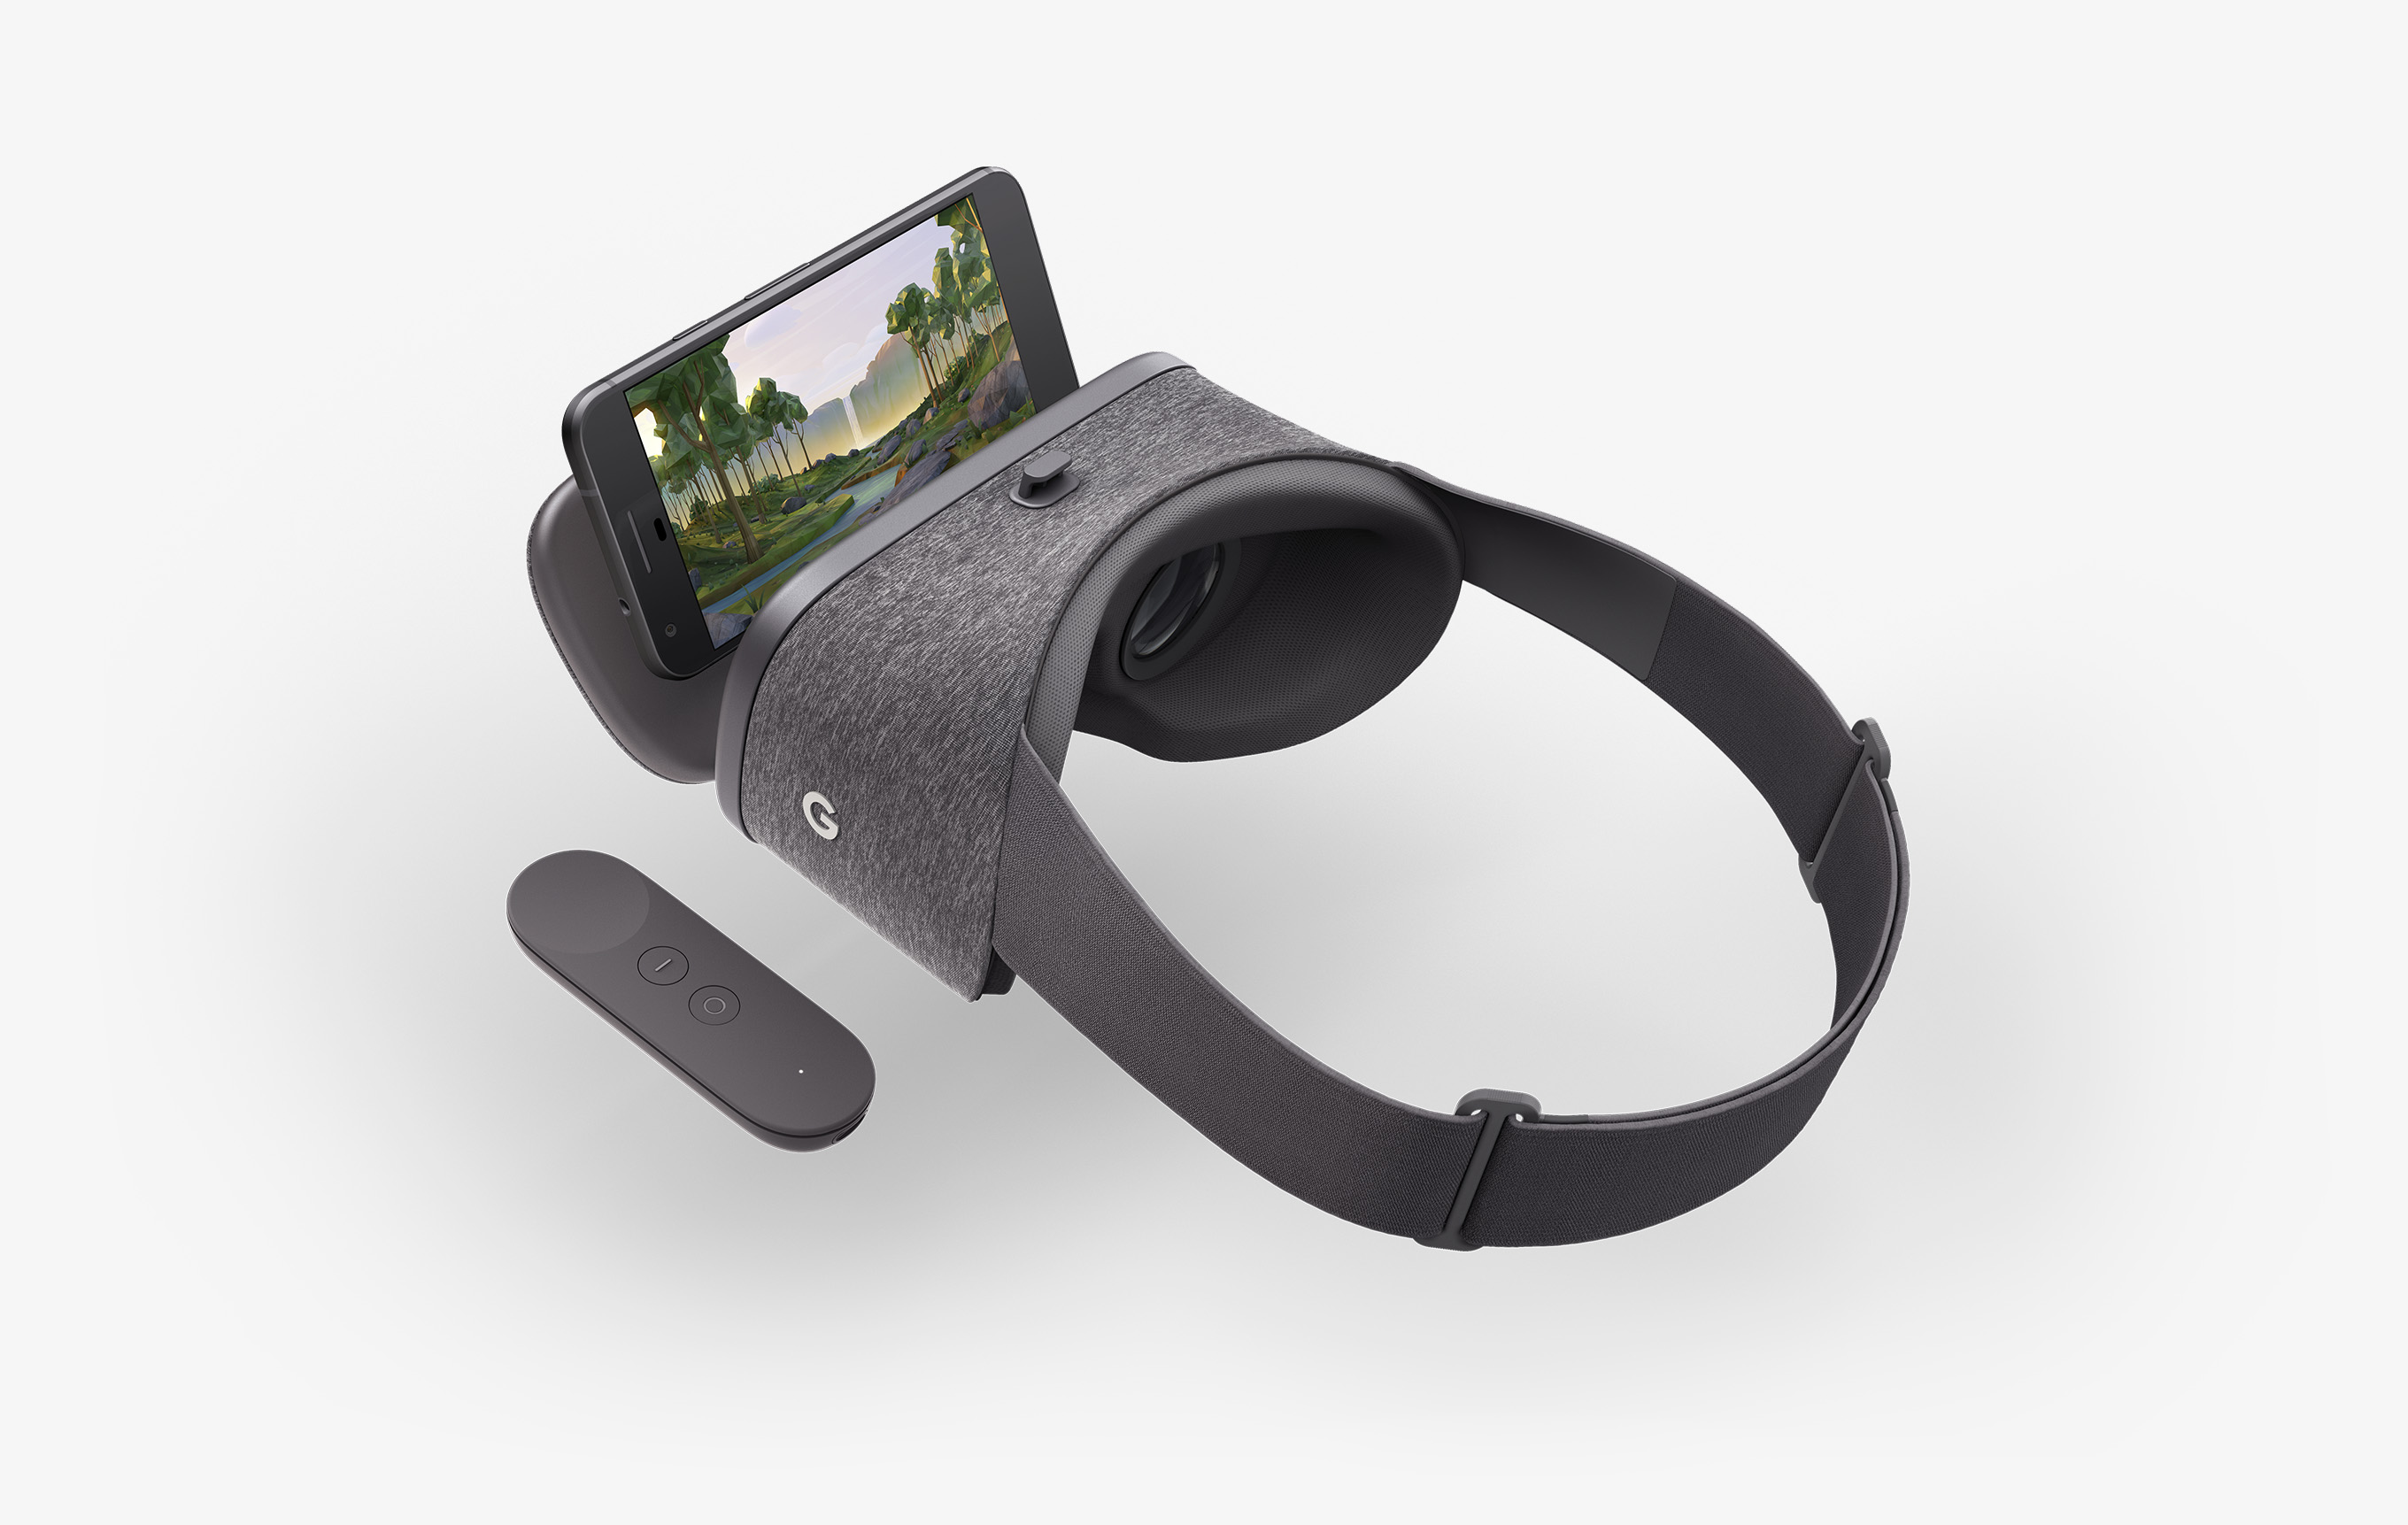
\includegraphics[scale=0.15]{Imagens/daydream.jpg}
	\label{f.daydream}
	\legend{\small Fonte: \cite{daydream}}
\end{figure}

As aplicações em RV podem ser desenvolvidas para plataformas mobile e desktop. A principal diferença entre as duas é a diferença de capacidade de processamento e memória, que são menores nos dispositivos móveis. Para as aplicações desktop utiliza-se óculos de RV como o Oculus Rift para executar a aplicação. Já nas aplicações para dispositivos móveis, é necessário um visualizador como o Google Cardboard por onde o smartphone será encaixado.

A fim de interagir com o ambiente virtual, o usuário pode utilizar a movimentação da cabeça e um controle externo como luvas, mouse 3D, joystick, entre outros. “A necessidade de se fazer uso de aparatos tecnológicos para a interação do usuário com o ambiente virtual provoca restrições, tanto pelo aspecto econômico e tecnológico, quanto pelo desconforto, mas permite ao usuário fazer coisas que antes eram impossíveis ou inviáveis. ” \cite[p. ~3]{torilivro}

Este projeto utiliza óculos de RV e um dispositivo móvel para criar uma aplicação que explora os conceitos da realidade virtual visando explorar diferentes formas de controle de interação.

